\section{Casos exatos, fases diádicas e validação}
\label{sec:dyadic-exact-cases}

\subsection{Curvatura constante: resposta completa}

\begin{theorem}[lei exata e intervalo de acumulação]
\label{thm:quadratic-dyadic-constant}
Se $K$ é uma célula diádica de comprimento $L$ e
$q''\equiv\kappa\ne0$ em $K$, ponha
\begin{equation}
 A=\frac{|\kappa|L^2}{8}.
 \label{eq:quadratic-A}
\end{equation}
Então, para todo $N\ge1$,
\begin{equation}
 E_N^{\rm dia}(q)_\infty
 =A\,4^{-\lfloor\log_2N\rfloor}.
 \label{eq:quadratic-exact-law}
\end{equation}
Consequentemente,
\begin{equation}
 \liminf_{N\to\infty}N^2E_N^{\rm dia}(q)_\infty=A,
 \qquad
 \limsup_{N\to\infty}N^2E_N^{\rm dia}(q)_\infty=4A,
 \label{eq:quadratic-liminf-limsup}
\end{equation}
e o conjunto completo dos valores de acumulação de
$N^2E_N^{\rm dia}(q)_\infty$ é o intervalo $[A,4A]$. Em particular, a
constante obtida por um limite simples não existe.
\end{theorem}

\begin{proof}
Em uma folha $J$ de comprimento $\ell$,
\begin{equation}
 e_q(J)=\frac{|\kappa|}{8}\ell^2.
 \label{eq:quadratic-local-exact}
\end{equation}
Se $r=\lfloor\log_2N\rfloor$, a árvore uniforme de profundidade $r$ usa
$2^r\le N$ folhas, todas de comprimento $L2^{-r}$, e atinge o lado direito
de \eqref{eq:quadratic-exact-law}. Para obter erro estritamente menor seria
necessário que toda célula da profundidade $r$ fosse subdividida, pois
qualquer uma mantida como folha ainda teria o erro de
\eqref{eq:quadratic-exact-law}. Isso exigiria $2^{r+1}>N$ folhas. A fórmula
está provada.

Agora
\[
 N^2E_N^{\rm dia}=A\left(\frac{N}{2^r}\right)^2,
 \qquad 2^r\le N<2^{r+1}.
\]
As escolhas $N=2^r$ e $N=2^{r+1}-1$ dão os extremos de
\eqref{eq:quadratic-liminf-limsup}. Para qualquer $t\in[1,2)$, tomar
$N_r=\lfloor t2^r\rfloor$ produz o limite $At^2$; o valor $4A$ é obtido
pela segunda sequência. Isso dá exatamente $[A,4A]$.
\end{proof}

Como $I(q)=L\sqrt{|\kappa|}$, os extremos são
$A=I(q)^2/8$ e $4A=I(q)^2/2$. Logo ambas as constantes do
\cref{thm:general-dyadic-envelope} são agudas. Em contraste, a referência de
nós livres tem a constante inferior $I(q)^2/8$: a restrição diádica a
recupera nas potências de dois, mas perde um fator que tende a quatro logo
antes da potência seguinte.

A formulação dual em tolerância também é exata:
\begin{equation}
 n_q(\varepsilon)
 =2^{\max\{0,\lceil\log_4(A/\varepsilon)\rceil\}}.
 \label{eq:quadratic-threshold-count}
\end{equation}
Ela fornece a contagem exata do ótimo interpolatório e coincide, em curvatura
constante, com a lei de refinamento certificado da \cref{sec:adaptive}.

\begin{table}[t]
 \centering
 \caption{Lei exata para $q(x)=x^2$ em $[0,1]$, quando $A=1/4$.}
 \label{tab:quadratic-exact}
 \small
 \begin{tabular}{rrrr}
\toprule
$N$ & $\lfloor\log_2N\rfloor$ & $E_N^{\rm dia}(q)_\infty$ & $N^2E_N/A$ \\
\midrule
1 & 0 & $\frac{1}{4}$ & 1.000000 \\
2 & 1 & $\frac{1}{16}$ & 1.000000 \\
3 & 1 & $\frac{1}{16}$ & 2.250000 \\
4 & 2 & $\frac{1}{64}$ & 1.000000 \\
7 & 2 & $\frac{1}{64}$ & 3.062500 \\
8 & 3 & $\frac{1}{256}$ & 1.000000 \\
15 & 3 & $\frac{1}{256}$ & 3.515625 \\
16 & 4 & $\frac{1}{1024}$ & 1.000000 \\
31 & 4 & $\frac{1}{1024}$ & 3.753906 \\
\bottomrule
\end{tabular}

\end{table}

\begin{figure}[t]
 \centering
 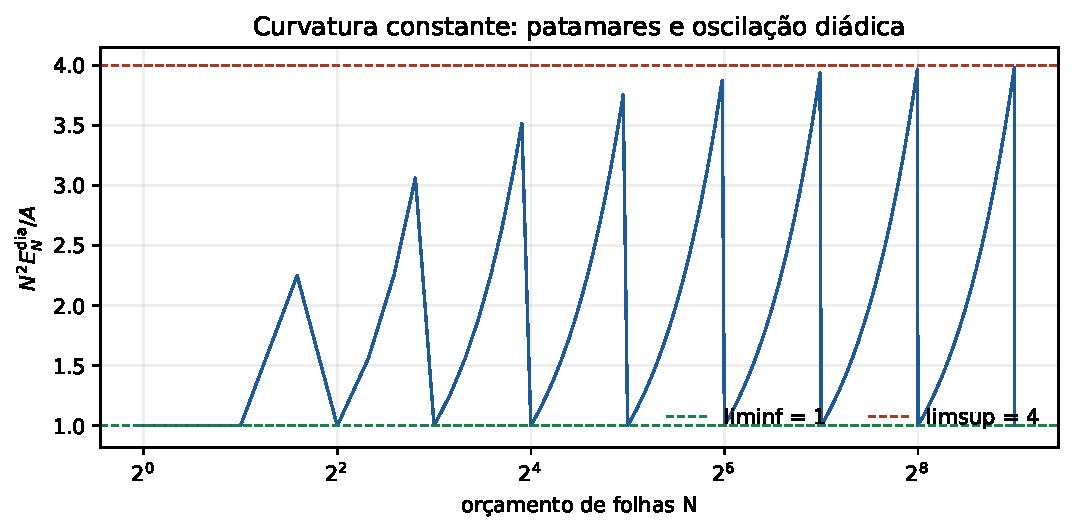
\includegraphics[width=.88\linewidth]{fig03_constante_quadratica.pdf}
 \caption{A normalização $N^2E_N^{\rm dia}/A$ reinicia em $1$ nas potências
 de dois e se aproxima de $4$ antes da potência seguinte.}
 \label{fig:quadratic-sawtooth}
\end{figure}

A \cref{tab:quadratic-exact} lista os valores racionais da lei, e a
\cref{fig:quadratic-sawtooth} exibe a oscilação normalizada entre as fases
diádicas consecutivas.

\subsection{Quadráticas por partes e lei de fase}

O caso seguinte separa a oscilação causada por uma única escala daquela
produzida por regiões com curvaturas diferentes.

\begin{theorem}[contagem exata em uma malha diádica base]
\label{thm:piecewise-quadratic-count}
Seja $\mathcal Q_{q_0}$ a partição uniforme de $K=[0,1]$ em células
$Q_i$ de comprimento $2^{-q_0}$. Suponha que $f\in C^1(K)$ seja quadrática
em cada $Q_i$ e
\[
 f''|_{\mathring Q_i}=\kappa_i\ne0,
 \qquad
 A_i=\frac{|\kappa_i||Q_i|^2}{8}.
\]
Existe $\varepsilon_0>0$ tal que, para
$0<\varepsilon<\varepsilon_0$,
\begin{equation}
 n_f(\varepsilon)
 =\sum_i2^{\lceil\log_4(A_i/\varepsilon)\rceil}.
 \label{eq:piecewise-count-law}
\end{equation}
Se $s=-\log_4\varepsilon$ e $a_i=\log_4A_i$, então
\begin{equation}
 \sqrt\varepsilon\,n_f(\varepsilon)
 =\Phi(s),
 \qquad
 \Phi(s)=\sum_i\sqrt{A_i}\,
 2^{\lceil s+a_i\rceil-(s+a_i)}.
 \label{eq:piecewise-phase-law}
\end{equation}
A função $\Phi$ é $1$-periódica e não constante. Portanto nem mesmo a
normalização em tolerância possui, em geral, um limite simples.
\end{theorem}

\begin{proof}
Todo ancestral da malha base que contém algum $Q_i$ é não afim, logo possui
erro local positivo. Como há apenas um número finito desses ancestrais,
escolha $\varepsilon_0$ menor que todos os seus erros e que todos os $A_i$.
O \cref{thm:threshold-optimality} obriga então a árvore de limiar a alcançar
cada $Q_i$. Dentro de $Q_i$, a identidade
\eqref{eq:quadratic-local-exact} mostra que são necessárias e suficientes
$2^{\lceil\log_4(A_i/\varepsilon)\rceil}$ folhas. Somar prova
\eqref{eq:piecewise-count-law}; a reescrita algébrica dá
\eqref{eq:piecewise-phase-law}. A periodicidade segue de
$\lceil s+1+a_i\rceil-(s+1+a_i)=\lceil s+a_i\rceil-(s+a_i)$.
Em qualquer intervalo aberto sem uma das finitíssimas fases de salto, todos
os tetos permanecem fixos e $\Phi$ é um múltiplo positivo de $2^{-s}$;
portanto é estritamente decrescente ali e não pode ser constante.
\end{proof}

\begin{corollary}[fases sincronizadas]
\label{cor:synchronized-phases}
Nas hipóteses do \cref{thm:piecewise-quadratic-count}, suponha ainda que
$A_i/A_j\in4^{\mathbb Z}$ para todos $i,j$. Então
\begin{equation}
 \liminf_{N\to\infty}N^2E_N^{\rm dia}(f)_\infty=\frac{I(f)^2}{8},
 \qquad
 \limsup_{N\to\infty}N^2E_N^{\rm dia}(f)_\infty=\frac{I(f)^2}{2}.
 \label{eq:synchronized-extremes}
\end{equation}
\end{corollary}

\begin{proof}
Escreva $A_i=A_\ast4^{-\rho_i}$ com $\rho_i\in\mathbb Z$ e, após deslocar
todos os índices, $\rho_i\ge0$. Para $r\ge\max_i\rho_i$, a tolerância
$\varepsilon_r=A_\ast4^{-r}$ produz
\[
 n_r=\sum_i2^{r-\rho_i}=C2^r,
 \qquad C=\sum_i2^{-\rho_i},
\]
folhas, todas com erro exatamente $\varepsilon_r$. Assim,
$E_{n_r}^{\rm dia}=\varepsilon_r$. Para reduzir o máximo estritamente, é
necessário subdividir cada uma das $n_r$ folhas; logo
$E_{2n_r-1}^{\rm dia}=\varepsilon_r$. Finalmente,
\[
 \sqrt{A_\ast}C=\sum_i\sqrt{A_i}=\frac{I(f)}{\sqrt8}.
\]
As duas sequências de orçamentos dão os extremos de
\eqref{eq:synchronized-extremes}; o envelope geral impede valores externos.
\end{proof}

A presença de sinais diferentes entre os $\kappa_i$ não altera essas
fórmulas: os erros locais dependem de $|\kappa_i|$. Para uma função global
$C^2$, uma mudança de sinal passa por zeros e a lei finita por fases deixa de
ser literalmente aplicável, mas o \cref{thm:general-dyadic-envelope} continua
válido sem alteração.

\begin{figure}[t]
 \centering
 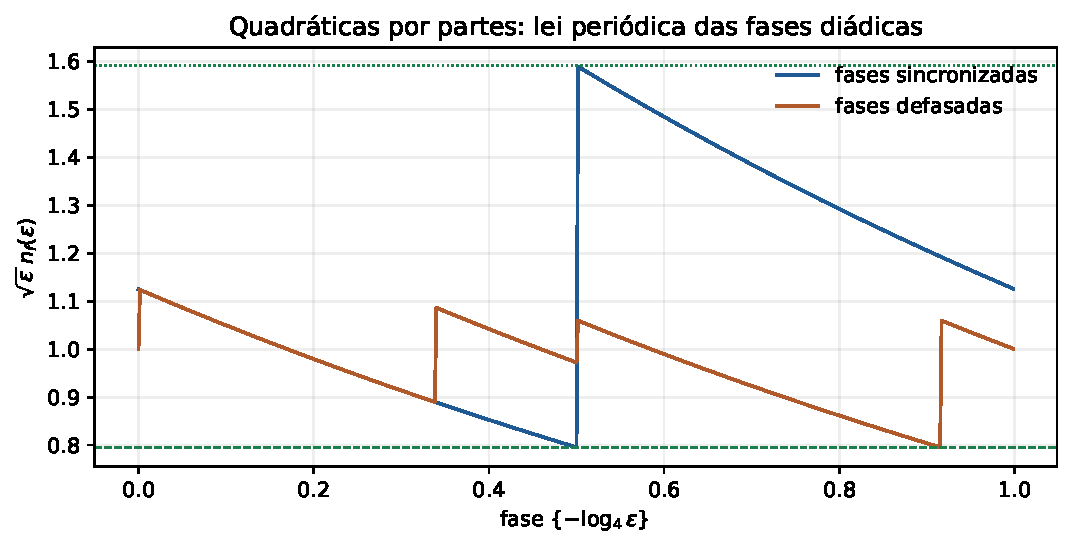
\includegraphics[width=.88\linewidth]{fig04_fases_piecewise.pdf}
 \caption{A lei \eqref{eq:piecewise-phase-law} em uma família sincronizada e
 outra defasada. Deslocar $-\log_4\varepsilon$ por uma unidade repete
 exatamente o perfil.}
 \label{fig:piecewise-phases}
\end{figure}

A sincronização e a defasagem previstas por
\eqref{eq:piecewise-phase-law} são comparadas na
\cref{fig:piecewise-phases}.

\subsection{Implementação e auditorias independentes}

O programa \texttt{constante\_diadica.py} implementa duas rotas que não
reutilizam a mesma recorrência: a árvore menos refinada do
\cref{thm:threshold-optimality} e uma programação dinâmica por número exato
de folhas,
\begin{equation}
 D(J,1)=e_f(J),\qquad
 D(J,n)=\min_{n_L+n_R=n}\max\{D(J_L,n_L),D(J_R,n_R)\}.
 \label{eq:independent-tree-dp}
\end{equation}
Para funções quadráticas por partes, $f$, $f'$, todos os pontos críticos e
todos os erros locais são calculados com \texttt{Fraction}. A fórmula
quadrática foi comparada com \eqref{eq:independent-tree-dp} para
$1\le N\le14$; a lei por partes foi confrontada com a construção explícita
do limiar em 14 escalas e a inversão do limiar foi comparada com a DP para
$1\le N\le12$.

Os dois diagnósticos $C^2$ usam apenas ponto flutuante determinístico para
avaliar extremos analíticos: $e^x$, cuja curvatura é estritamente positiva,
e $(x-1/2)^3$, cuja segunda derivada muda de sinal. Eles não participam de
nenhuma prova de igualdade; verificam apenas que os valores finitos
$\varepsilon n_f(\varepsilon)^2$ permanecem dentro do envelope teórico nas
$400$ tolerâncias examinadas.

\begin{remark}[agudeza uniforme e comportamento pontual]
\label{rem:envelope-not-pointwise}
O \cref{thm:general-dyadic-envelope} é agudo \emph{uniformemente sobre a
classe} $C^2$: a mesma função quadrática do
\cref{thm:quadratic-dyadic-constant} realiza $I(f)^2/8$ e $I(f)^2/2$ ao longo
de subsequências. Logo as duas constantes são ótimas em teoremas uniformes
sobre $C^2$. Para uma função fixa, o conjunto de acumulação pode ser um
subconjunto próprio do envelope.

No modelo finito do \cref{thm:piecewise-quadratic-count}, essa distinção pode
ser tornada exata. Ponha $w_i=\sqrt{A_i}$ e considere os resíduos de
$a_i=\log_4A_i$ módulo $1$. Cada fator
\[
 g(s+a_i)=2^{\lceil s+a_i\rceil-(s+a_i)}
\]
pertence a $[1,2)$ e vale $1$ precisamente quando $s+a_i\in\mathbb Z$. Se os
resíduos não são todos iguais, não existe fase que torne simultaneamente
todos os fatores iguais a $1$, nem uma sequência de fases que os faça tender
simultaneamente a $2$. Como há apenas um número finito de fases de salto no
círculo, existem $\delta_-,\delta_+>0$ tais que
\[
 \frac{I(f)}{\sqrt8}+\delta_-
 \le \Phi(s)
 \le \frac{I(f)}{\sqrt2}-\delta_+
 \qquad(s\in\mathbb R).
\]
Assim, a normalização dual $\varepsilon n_f(\varepsilon)^2$ permanece
estritamente dentro do envelope para todas as tolerâncias suficientemente
pequenas nessa família defasada. No caso sincronizado, a condição
$A_i/A_j\in4^{\mathbb Z}$ do \cref{cor:synchronized-phases} alinha os
resíduos e permite recuperar os extremos.

A prova finita usa o número discreto de fases de salto e, portanto, é
específica da curvatura quadrática por partes. A
\cref{tab:smooth-diagnostics} registra que, em $400$ tolerâncias entre
$10^{-3}$ e $10^{-10}$, os dois exemplos suaves permanecem estritamente no
interior. A caracterização, para $f$ dada, do conjunto exato de acumulação de
$N^2E_N^{\rm dia}(f)_\infty$ dentro de
$[I(f)^2/8,I(f)^2/2]$ constitui o problema de fases para curvatura variável.
\end{remark}

\begin{table}[t]
 \centering
 \caption{Diagnósticos determinísticos em 400 tolerâncias entre
 $10^{-3}$ e $10^{-10}$. As colunas externas são teóricas.}
 \label{tab:smooth-diagnostics}
 \small
 \begin{tabular}{lrrr}
\toprule
função & $I(f)^2/8$ & faixa observada de $\varepsilon n_f(\varepsilon)^2$ & $I(f)^2/2$ \\
\midrule
$e^x$ & 0.210420 & [0.339008, 0.515293] & 0.841679 \\
$(x-\frac{1}{2})^3$ & 0.166667 & [0.275877, 0.417099] & 0.666667 \\
\bottomrule
\end{tabular}

\end{table}

\begin{figure}[t]
 \centering
 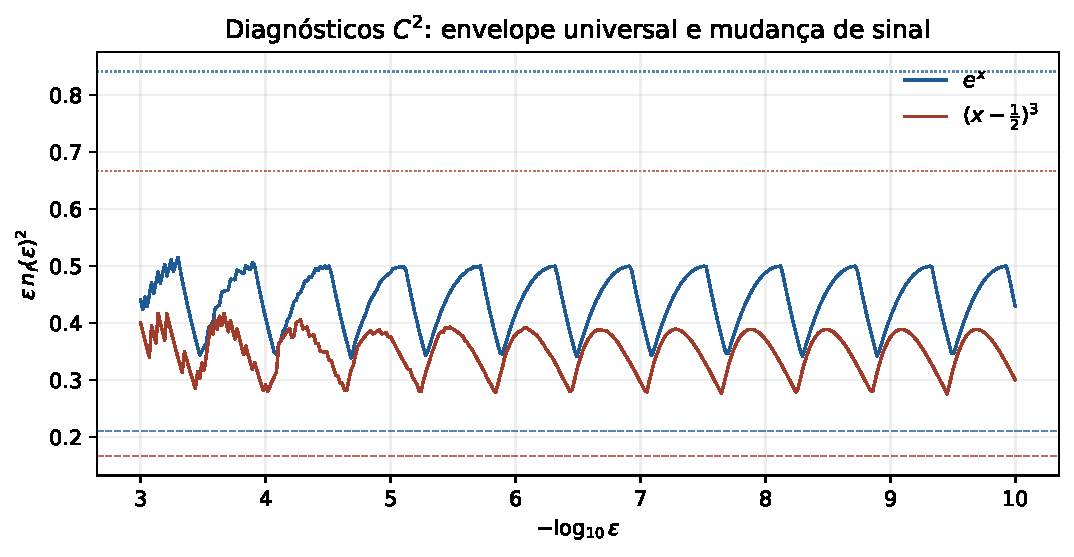
\includegraphics[width=.88\linewidth]{fig05_envelope_c2.pdf}
 \caption{Diagnósticos para curvatura positiva e para mudança de sinal. As
 linhas tracejadas e pontilhadas são, respectivamente, $I(f)^2/8$ e
 $I(f)^2/2$.}
 \label{fig:c2-envelope}
\end{figure}

Os dois exemplos suaves da \cref{fig:c2-envelope} permanecem dentro do
envelope teórico em todas as tolerâncias auditadas.

\begin{table}[t]
 \centering
 \caption{Auditoria executável das constantes diádicas.}
 \label{tab:dyadic-constants-audit}
 \small
 \begin{tabularx}{\linewidth}{@{}Xr@{}}
\toprule
Verificação & resultado \\
\midrule
Fórmula quadrática $=$ DP independente & true \\
Limiar quadrático $=$ contagem fechada & true \\
Contagem por partes $=$ árvore de limiar & true \\
DP por partes $=$ inversão do limiar & true \\
Fases sincronizadas atingem os dois extremos & true \\
Diagnóstico $C^2$ positivo dentro do envelope & true \\
Mudança de sinal dentro do envelope & true \\
Varreduras suaves estritamente interiores (400 pontos) & true \\
Execução sem números pseudoaleatórios & true \\
\bottomrule
\end{tabularx}

\end{table}

A \cref{tab:dyadic-constants-audit} reúne, em uma única trilha, as
identidades exatas e os testes independentes desta seção.

\subsection{Compatibilidade com a altura aritmética}

Os teoremas desta seção permitem todos os descendentes da raiz. Na biblioteca
$\Library$, uma malha uniforme de profundidade relativa $r$ em
$K=J_{k_0,m_0}$, $m_0\ge0$, só está espacialmente disponível quando
\[
 H\ge k_0+r+1,
 \qquad H\ge2^r(m_0+1)
\]
pela \cref{prop:translation-obstruction}. Como as escalas relevantes têm
$2^r\asymp N$, a segunda condição já força $H=\Omega(N(m_0+1))$, antes de
se contabilizar a altura necessária para racionalizar os valores nodais.
Assim, a passagem de \eqref{eq:budget-envelope} para uma agenda $H(N)$ inclui
esse acoplamento geométrico.

Para cada árvore fixa, o teorema de racionalização da \cref{sec:assemblies}
aproxima os valores nodais reais por racionais compartilhados e aproxima
$P_\Lambda f$ arbitrariamente bem por uma montagem da biblioteca. Os
interpolantes pertencem, portanto, à aderência quando a altura cresce. O
problema interpolatório \eqref{eq:optimal-dyadic-interpolation} e o melhor
erro racional com deslocamentos nodais são objetos distintos; a constante
assintótica do segundo sob uma agenda fixa de altura permanece em aberto.
